\section{Ejercicio 7}
\subsection{Desarrollo}
Analizamos con varios grupos de tareas el comportamiento de $SchedMistery$ para llegar a los siguientes resultados. Llamar\'e E a las entradas.

\begin{enumerate}[(a)]

\item $SchedMistery$ es un scheduler de Multiples Colas con prioridad.

\item Siendo N la cantidad de entradas que se le da al programa (\#E), el SchedMistery tendr\'a N+1 colas de prioridad, siendo la primera de 1 tick y el quantum del resto corresponde a los valores ingresados.

\item La cola de quantum 1 es la de mayor prioridad y el resto de colas va decendiendo su prioridad en el orden que se ingresan.

Ej: Siendo prioridad N+1 la m\'as alta
\begin{table}[H]
\centering
\begin{tabular}{ | c | c | c |}
  \hline			
  Cola N$^{ro}$ & quantum & prioridad\\
  \hline
1 	& 1 			& N+1\\
2 	& $E_1$ 		& N\\
3 	& $E_2$ 		& N-1\\
4 	& $E_3$ 		& N-2\\
5 	& $E_4$ 		& N-3\\
  \hline
i 	& $E_{i-1}$ 	& N-i+2\\
  \hline
N+1 & $E_N$ 		& 1\\
  \hline

\end{tabular}
\end{table}

\item Siempre se ejecutan las tareas de la cola no vac\'ia de menor prioridad.

\item Si una tarea corre el quantum completo (i.e. no se bloquea o termina) y hay una cola de prioridad menor, la tarea es eliminada de la cola E$_i$ en la que se encuentra y pasa a la cola E$_{i+1}$.\\
	Si estaba en la cola de prioridad 1 (i.e. la \'ultima cola), se queda en ella.
	
\item Las tareas que corren el quantum completo en la \'ultima cola pasan al final de la cola, funcionando como un $Round Robin$ con el quantum de la \'ultima cola.
	
\item Si una tarea es bloqueada, es eliminada de la cola en la que se encuentra y pasa a la cola E$_{i-1}$ salvo que se encuentre en la primer cola. En cuyo caso se la vuelve a agregar al final de la misma.

\end{enumerate}

Para hacer SchedNoMistery utilizamos un vector de colas, de nombre tareas, y otro vector de quantums. Tienen el mismo tamaño y están balanceados el uno con el otro, es decir que si accedes a la posición i de tareas en la misma de quantums estará el tiempo de procesador de la cola. 

Luego tenemos una estructura tarea que consiste en el pid del proceso y el índice de la cola a la que pertenece en tareas. Tendremos una tarea de nombre Actual, que es la que está corriendo, el quantum restante de la misma. Y por ultimo un vector de tarea que contiene las tareas que están actualmente bloqueadas, esta tiene el nombre de bloqueados.

El proceso load lo que hará es sencillamente crear la nueva tarea y encolarla en la primera cola(mayor prioridad)

Por otro lado, unblock se encargará de buscar el pid dado en el vector bloqueados y, cuando lo encuentra, lo quita de allí. La estructura tarea obtenida ahora debe ser pasada a la cola anterior a la que se encontraba cuando fue bloqueada (si es que no es la primera, en cuyo caso se queda en la misma).

Para terminar, tenemos tick. Para los tres motivos esto es lo que hace:

TICK: Si todavía me queda quantum en la tarea actual entonces disminuyo este en 1 y retorno el pid de Actual. Si no es el caso entonces, guardo la tarea en la siguiente cola a la que estaba (si es que la hay). Busco entre las colas de tareas la primera que no esté vacía y pongo esa tarea a ejecutar. En el caso que no aya simplemente le pongo a la actual el pid de IDLE y de quantum 0.

 BLOCK: Si la tarea no se encontraba bloqueada, la añado al vector bloqueados. Después repito el ultimo paso de TICK y me fijo si hay alguien para ejecutar.

EXIT: Hago lo mismo que los anteriores al final y me fijo si hay alguien para ejecutar.



\subsection{Experimentación}

\begin{comment}
Ahora mostraremos de donde obtuvimos la información antes mencionada

Los lotes utilizados fueron:\\

loteEj7a.tsk\\
TaskCPU 18\\
TaskCPU 18\\
TaskCPU 18\\
TaskCPU 18\\


loteEj7b.tsk\\
\#Tarea intensiva de CPU 1\\
TaskCPU 18\\
\#Tarea intensiva de CPU 2\\
@7:\\
TaskCPU 20\\
\#Tarea interactiva 1\\
TaskConsola 4 3 6\\
\#Tarea interactiva 2\\
TaskConsola 8 2 7 \\





\begin{figure}[H]
  \centering
    %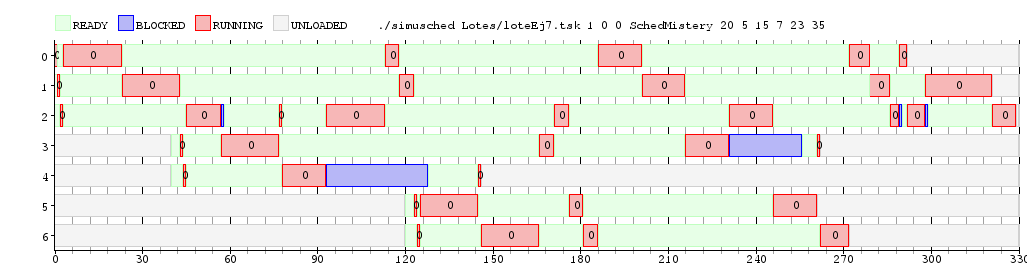
\includegraphics[width=1.1\textwidth]{imagenes/test1ej7.png}
  \caption{Se pueden apreciar (a)(b)(e)(f)}
  \label{fig:ej7a}
\end{figure}

En esta figura se puede ver claramente que es un Round Robin y que los tiempos que toman las tareas cada vez que entran en Ready son 1, 3, 2, 4, 4.. Luego de la cuarta vez que el scheduller pone a correr la tarea, siempre le da 4 tics de reloj


\begin{figure}[H]
  \centering
    %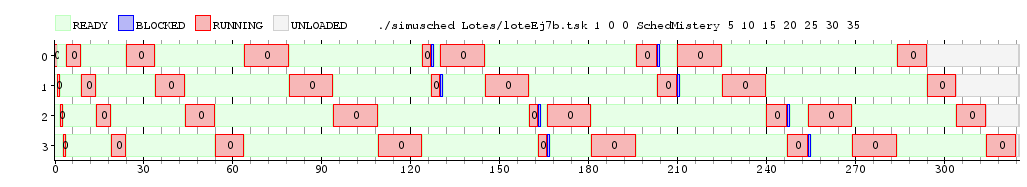
\includegraphics[width=1.1\textwidth]{imagenes/test2ej7.png}
  \caption{Se pueden apreciar (a)(b)(d)}
  \label{fig:test2ej7}
\end{figure}


\begin{figure}[H]
  \centering
    %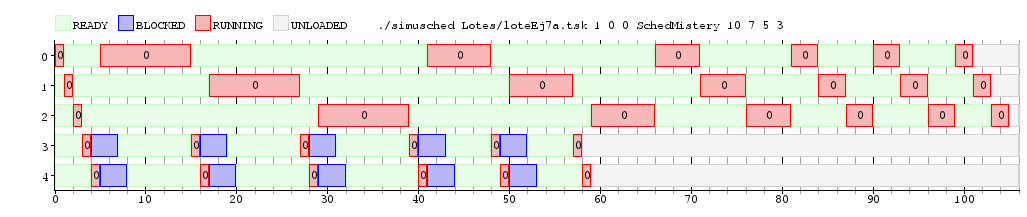
\includegraphics[width=1.1\textwidth]{imagenes/test3ej7.png}
  \caption{Se pueden apreciar (a)(b)(c)(e)(f)(g)}
  \label{fig:test3ej7}
\end{figure}
\end{comment}
